\begin{figure}[ht]
  \begin{center}
    \newlength{\zl}
\settowidth{\zl}{$_0$}
%%\the\zl
\psfrag{0.1}{\raisebox{-2pt}{0.01}}
\Large
\psfrag{ T1}{ $g_{10}$ \hspace{23.51387pt}\psline(0,0)(4.5,0)}
\psfrag{ T2}{ $g_9$ \hspace{28pt}\psline(0,0)(4.5,0)}
\psfrag{ T3}{ $g_8$ \hspace{28pt}\psline(0,0)(4.5,0)}
\psfrag{ T4}{ $g_7$ \hspace{28pt}\psline(0,0)(4.5,0)\rput(-7.5,0){\raisebox{8pt}{$\mathcal{N}$}}}
\psfrag{ T5}{ $g_6$ \hspace{28pt}\psline(0,0)(4.5,0)}
\psfrag{ T6}{ $g_5$ \hspace{28pt}\psline(0,0)(5,0)\psframe[fillstyle=solid,fillcolor=gray](2.25,-0.1)(2.75,0.1)}
\psfrag{ T7}{ $g_4$ \hspace{28pt}\psline(0,0)(5,0)\psframe[fillstyle=solid,fillcolor=gray](2.25,-0.1)(2.75,0.1)}
\psfrag{ T8}{ $g_3$ \hspace{28pt}\psline(0,0)(5,0)\psframe[fillstyle=solid,fillcolor=gray](2.25,-0.1)(2.75,0.1)\rput(-7.5,0){\raisebox{2pt}{$\mathcal{T}$}}}
\psfrag{ T9}{ $g_2$ \hspace{28pt}\psline(0,0)(5,0)\psframe[fillstyle=solid,fillcolor=gray](2.25,-0.1)(2.75,0.1)}
\psfrag{ T10}{ $g_{1}$ \hspace{28pt}\psline(0,0)(5,0)\psframe[fillstyle=solid,fillcolor=gray](2.25,-0.1)(2.75,0.1)}

\hspace{-2.8cm}\scalebox{0.6}{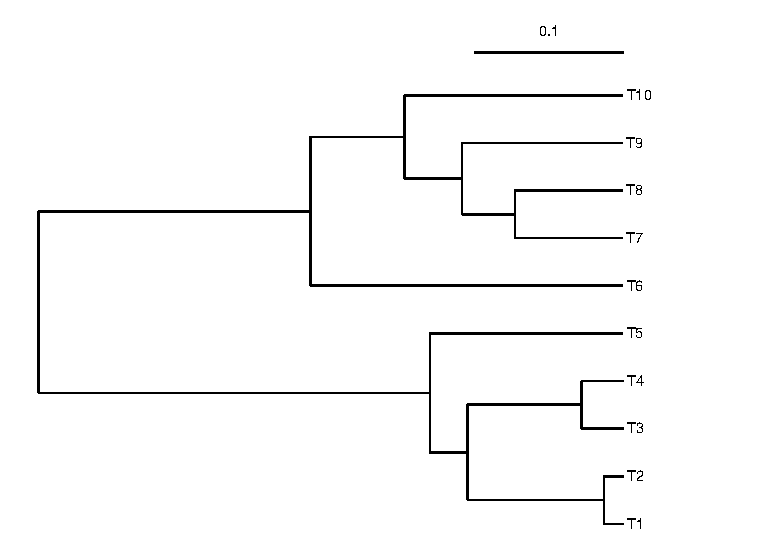
\includegraphics{tn}}
\end{center}
\caption{The program \ty{stan} simulates a genealogy of targets,
  $\mathcal{T}$, and neighbors, $\mathcal{N}$. It then simulates
  genomes sequences along this phylogeny. The targets contain a marker
  region (gray) that is deleted in the neighbors. This region is
  searched for by tools for neighbor-based marker
  design.}\label{fig:tn}
\end{figure}

Diagnostic genetic markers are developed from sequence regions that
are present in all targets and absent from all other sequences. This
absence from all other sequences helps to ensure that the markers do
not cross-react. Since the vast majority of cross-reacting sequences
of a set of target strains are contained in the closest phylogenetic
neighbors, subtraction of neighbors from targets is a useful first
step when designing markers.

Programs for such neighbor-based marker design thus start from a set
of target sequences and a set of neighbor sequences and determine the
regions present in all targets and absent from all
neighbors. Figure~\ref{fig:tn} is a cartoon of the phylogeny of five
target genomes, $\mathcal{T}$, and five neighbor genomes,
$\mathcal{N}$. The target genomes contain two common regions that are
absent from the neighbors. The absence from the neighbors is achieved
either through deletion or mutation. Such regions make good starting
material for marker development. The program Fur for \emph{find unique
regions} is an example of a program for efficient neighbor-based
extraction of marker regions from genome
sequences~\cite{hau21:fur}.

Like any estimation procedure, programs for neighbor-based extraction
of marker regions work under a model. This model can in turn be used
to simulate data for testing programs for neighbor-based marker
extraction. Performing well on such simulated data is a necessary
condition for application to real data, where the complications are
usually much greater. Here I write the program \ty{stan} for
simulating target and neighbor sequences.

In \ty{stan} we construct a coalescent tree where the deepest split is
between targets and neighbors. We then simulate sequences along that
coalescent and delete marker regions from the neighbors. Finally, the
target and the neighbor sequences are written to into separate files
in separate directories.

The deletions created by \ty{stan} are set by the user and affect all
neighbors equally. To generate more complicated deletion patterns, I
also supply the program \ty{rad}, for ``random deletion''. The program
\ty{rad} takes as input a sequence and deletes a Poisson-distributed
number of regions of normally-distributed lengths.
